\documentclass{article}
\usepackage{times}
\usepackage{amsmath}
\usepackage{amsfonts}
\usepackage{fancyhdr}
\usepackage{amssymb}
\usepackage{tabularx}
\usepackage{listings}
\usepackage{graphicx}
\usepackage{enumerate}
\usepackage{cite}
\usepackage{amsthm}
\usepackage{color}
\usepackage{soul}
\usepackage[bookmarks,colorlinks=true,linkcolor=black,citecolor=black,urlcolor=blue]{hyperref}
\usepackage{authblk}
\usepackage{placeins}
\usepackage{longtable}

\begin{document}

\title{IP-Controlled Low Voltage DC\\Power Distribution Unit\\ADVANCE DATASHEET}
\author{Andrew Zonenberg\\
	\texttt{azonenberg@drawersteak.com}}
\date{\today}
\maketitle

\fancyhead[L]{ADVANCE DATASHEET}
\fancyfoot[L]{$Revision$ / \today}
\pagestyle{fancy}

\setcounter{tocdepth}{2}
\tableofcontents

\pagebreak
\section{Introduction}

\subsection{Overview}
The PDU is an intelligent power distribution system for a large number (up to ten) of low voltage DC loads, such as 
encountered in a development board cluster for embedded prototyping. It is intended to consolidate many ``wall wart" 
power supplies into a single unit supplied by an external high-efficiency supply, saving outlet and workbench space 
while providing additional management and safety capabilities.

This is an advance specification of a system which is still under development. Some specifications are subject to 
change. Data marked as ``TBD" is dependent on characterization of prototype hardware.

\subsection{Feature summary}

\begin{itemize}
\item All functions of the device are accessible via SNMP using the on-board 10/100/1000 Mbps Ethernet port.
\item Each output channel is individually switched to permit remote reset of a malfunctioning DUT.
\item Per-channel current metering allows real-time monitoring of current consumed by downstream loads, providing
instant feedback when optimizing DUT firmware for power.
\item Board-level reverse voltage protection guards against incorrect hookup of the upstream supply.
\item Input rail voltage is monitored internally and all outputs are disabled if the voltage deviates from nominal by 
more than a set threshold. A jumper on the board allows 5V or 12V mode to be selected and prevents damaging downstream 
devices if the PDU is accidentally connected to the wrong supply.
\item Two chassis temperature monitors allow thermal shutdown in the event of overload.
\item Programmable overcurrent shutdown for extremely rapid ($\mu s$ or less) shutdown of a shorting or malfunctioning
DUT. This protection responds significantly faster than a fuse and can be remotely reset once the fault condition has 
been cleared. Firmware allows flexible tailoring of overcurrent shutdown behavior including response time; a separate 
power-on threshold prevents false triggering from inrush currents.
\item Ten 3.3V  digital GPIO pins are provided for interfacing with external systems.
\item The entire system design (hardware and firmware) is released under a permissive open source license (3-clause
BSD). KiCAD design files and firmware source are available at \url{https://code.google.com/p/azonenberg-devboards/}
under the  subproject ``pdu-5v-20a". Modified firmware may be loaded onto the system via the provided JTAG header.
\end{itemize}

\pagebreak
\section{Theory of operation}

\subsection{System overview}

The PDU requires an external (off board) 5V / 12V DC supply which should be capable of supplying at least 20A 
continuously. Power from the external connector is fed through a high-side PMOS based reverse voltage protection 
circuit to the primary power rail, which has two parallel 4700 $\mu F$ capacitors on it to smooth out load transients.

A tap on the primary power rail supplies power through two DC-DC converters and a linear regulator to the 3.3 / 2.5 / 
1.2V rails used by the FPGA, Ethernet PHY, and other control logic.

The primary power rail is then split off to the ten output stages (described below) which each supplies two screw 
terminals on the output connector. Outputs are not isolated; the input supply and all outputs share the same ground 
with high-side switching.

\begin{figure}[h!]
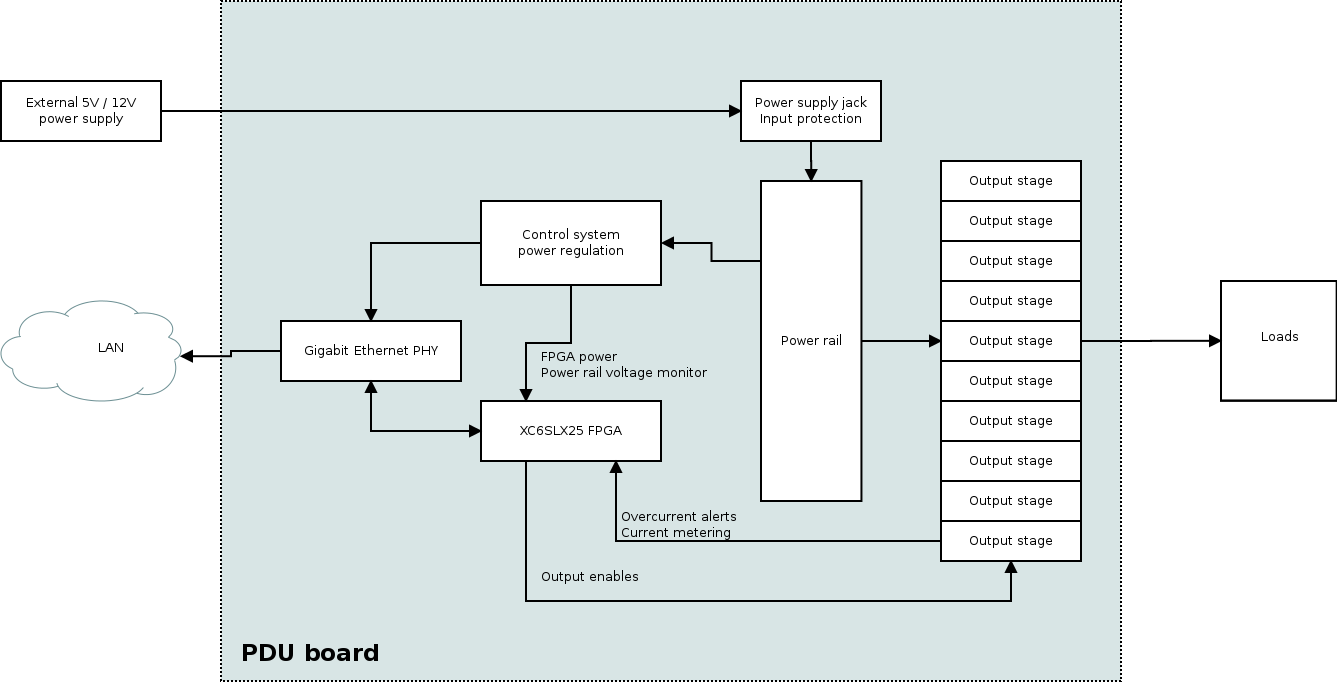
\includegraphics[scale=0.25]{system-block.png}
\caption{System block diagram}
\label{system-block}
\end{figure}
\FloatBarrier

\subsection{Output stage}

Each of the ten output channels is identically configured.

A 3.3V active-high output enable from the control logic is level-shifted to the power rail voltage by an N-channel
MOSFET, which then drives the gate of a high-side P-channel MOSFET. The switched power runs through a 5A fuse (as 
secondary protection in the event of an FPGA malfunction) and a ferrite chip to reduce coupling of EMI between 
downstream devices.The filtered power is then decoupled by a $150 \mu F$ electrolytic and $10 \mu F$ ceramic 
capacitor and fed through a $5 m\Omega$ shunt resistor to the output terminals.

\begin{figure}[h!]
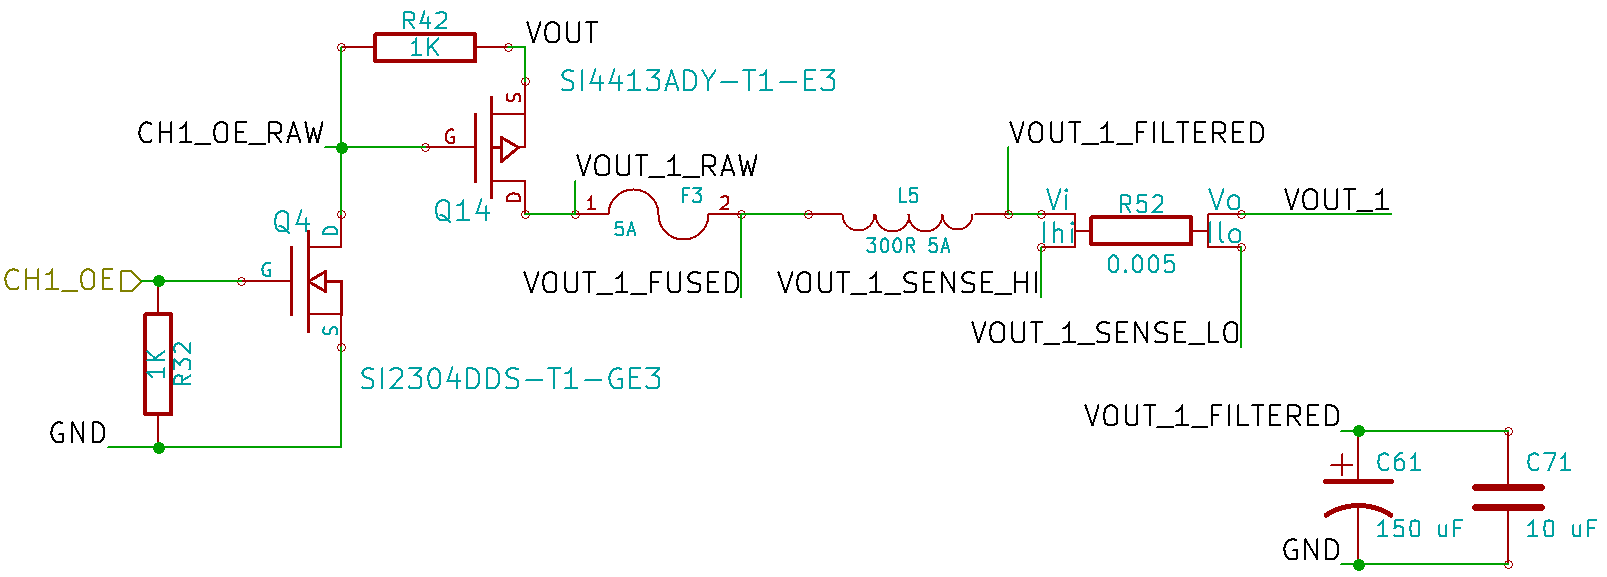
\includegraphics[scale=0.25]{output-stage-1.png}
\caption{Output stage circuit schematic}
\label{output-stage-1}
\end{figure}
\FloatBarrier

The shunt voltage is amplified 100x using by a Texas Instruments INA199A2 instrumentation amplifier to produce a 
voltage of 0.5V per A of output current and fed to a TLV3201 comparator. The resulting active-high overcurrent signal 
is sent to the FPGA, which will then shut down the output.

The comparator's reference voltage is supplied by a Texas Instruments DAC5573 8-bit DAC controlled over an I2C bus 
from the FPGA. One code value at the DAC corresponds to approximately 19.5 mA of current at the load. Note that the 
shunt resistor has a thermal coefficient of 50ppm and a tolerance of 1\%.

The stock firmware does not attempt to calibrate out ADC/DAC nonlinearity or shunt resistance variation, however the
FPGA has sufficient flash memory and block RAM to store per-board calibration values if required by custom firmware.

\begin{figure}[h!]
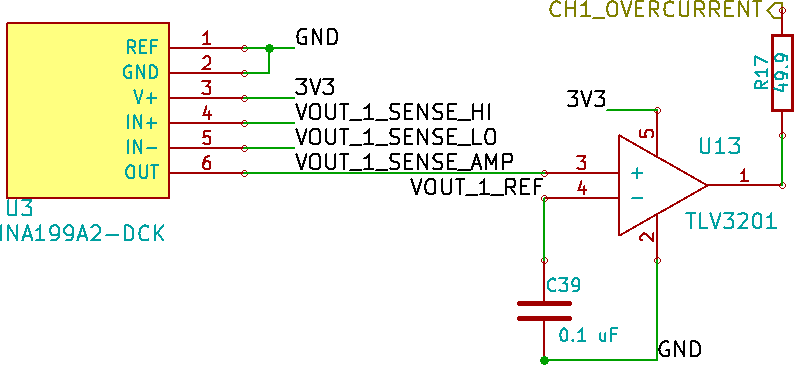
\includegraphics[scale=0.25]{output-stage-2.png}
\caption{Overcurrent detection circuit schematic}
\label{output-stage-2}
\end{figure}

Three Microchip MCP3204 12-bit 4-channel ADCs are connected to the amplified shunt voltage of each channel for metering
purposes, controlled by the FPGA over an SPI bus. A dedicated SPI bus is used for each of the three ADCs permitting
simultaneous sampling of of three values. The two remaining ADC channels are used to read the output rail voltage
(divided by four with 0.1\% tolerance $30K\Omega$ / $10K\Omega$ resistors to stay within the ADC's input range) at each
end of the power plane. One ADC code value corresponds to 1.22 mA at the load, or 2.44 mV of rail voltage.

\pagebreak
\section{Usage}

\subsection{External connections}

\subsection{Setup}

\subsection{Overcurrent protection}

The stock firmware includes delays to prevent high-frequency load transients from triggering an overcurrent 
shutdown. A 32-bit timer for each channel begins counting up at 100 MHz on the rising edge of the overcurrent alert 
signal and is reset on the falling edge. If the timer ever reaches the value of the CHx\_OVRCOUNT register, the 
output is disabled and the ``CHANNEL FAULT" LED is illuminated until the channel is manually turned off and then on 
again.

Optionally, a higher value for the overcurrent timer may be used immediately after the channel is turned on, to 
prevent inrush currents from triggering a shutdown. If the CHx\_STARTTIME register is nonzero, the overcurrent timer 
is compared against CHx\_INRUSHCOUNT rather than CHx\_OVRCOUNT for the first CHx\_STARTTIME cycles of the 100 MHz system
clock.

\pagebreak
\section{SNMP interface}

TODO: warn about setting OC limits $\geq$ 25A combined

\pagebreak
\section{Mechanical characteristics}

Four mounting holes (4-40 clearance size), one near each corner, are provided for mounting the board on standoffs to a 
workbench or enclosure.

\begin{figure}[h]
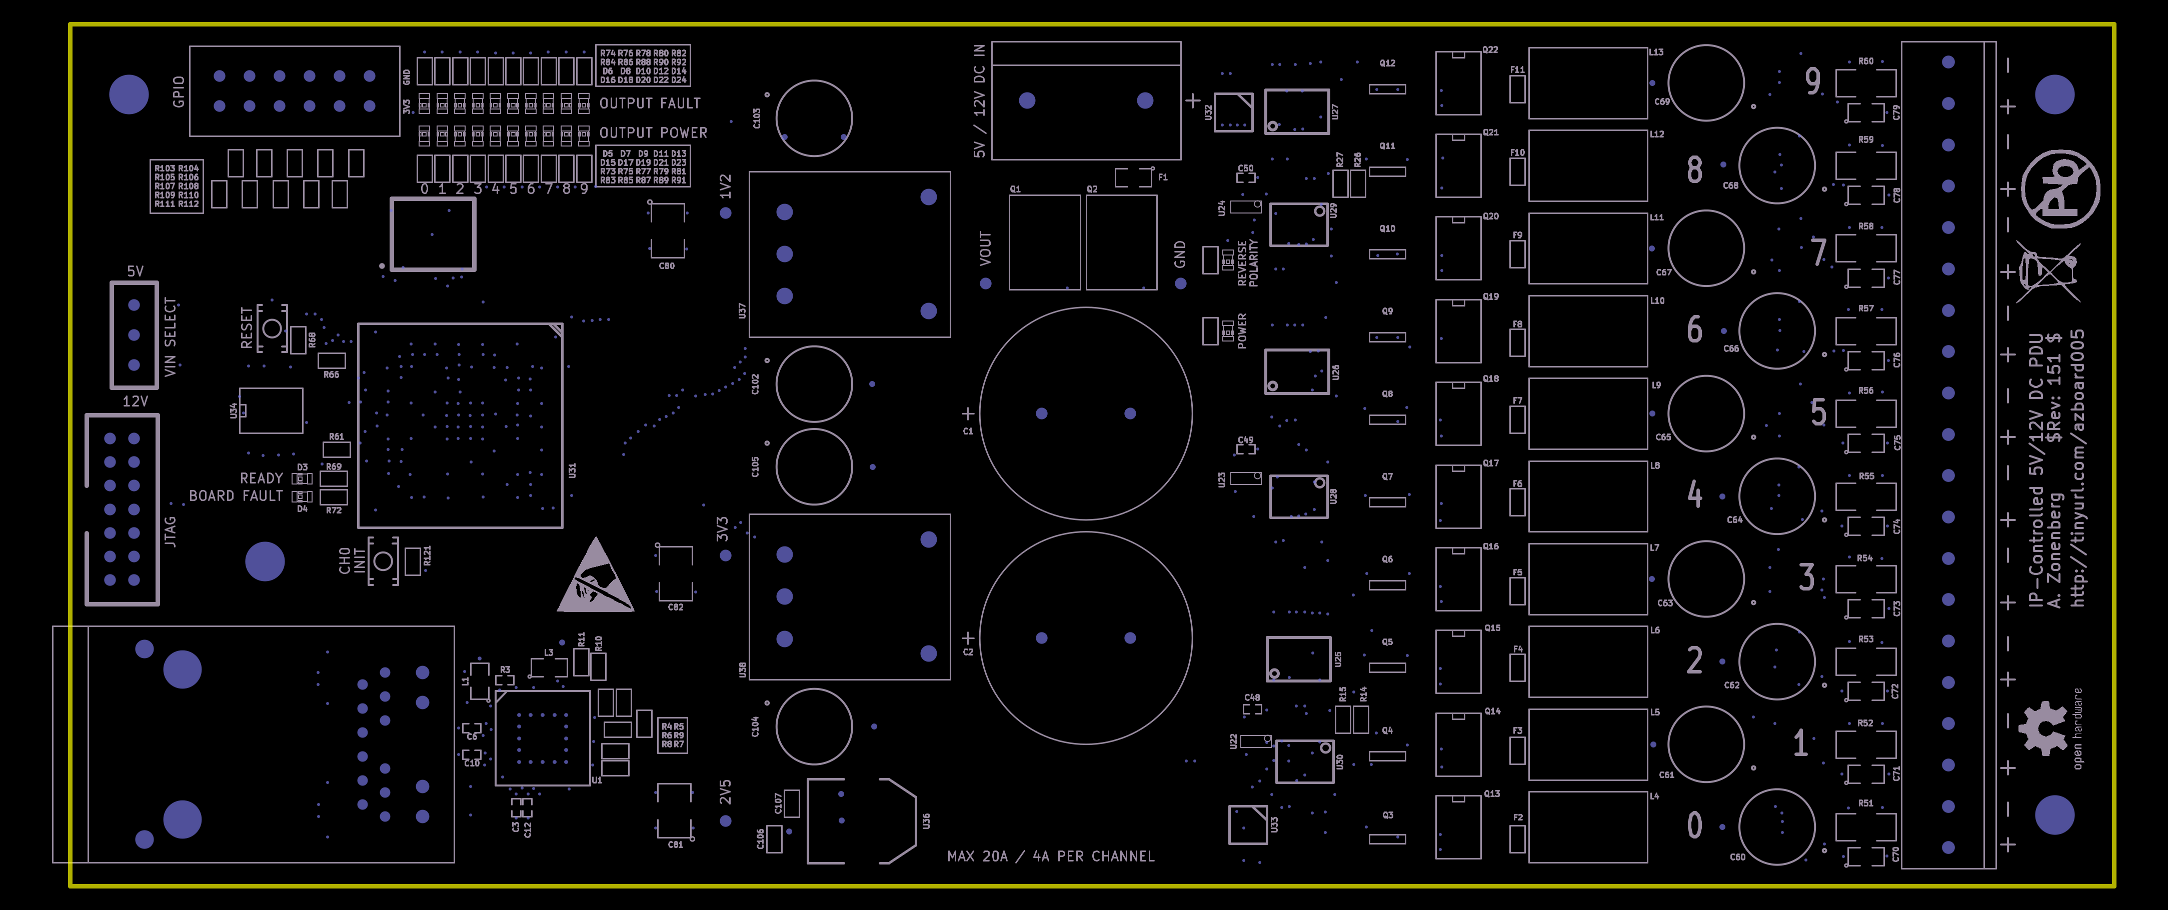
\includegraphics[scale=0.19]{silk-front-small.png}
\caption{PCB mechanical overview}
\label{silk-front}
\end{figure}

\begin{longtable}{|l|p{2in}|p{0.5in}|p{0.5in}|}
\hline
{\bf Symbol} & {\bf Description} & {\bf Typ} & {\bf Units}\\
\hline
$Len_{x}$ & Board size (horizontal axis) & 173 & mm\\
\hline
$Len_{y}$ & Board size (vertical axis) & 73 & mm\\
\hline
$DHole$ & Mounting hole diameter & 3.4 & mm\\
\hline
$Hole1_{x}$ & Mounting hole 1 X coordinate & 5.0 & mm\\
$Hole1_{y}$ & Mounting hole 1 Y coordinate & 6.0 & mm\\
\hline
$Hole2_{x}$ & Mounting hole 2 X coordinate & 16.5 & mm\\
$Hole2_{y}$ & Mounting hole 2 Y coordinate & 45.5 & mm\\
\hline
$Hole3_{x}$ & Mounting hole 3 X coordinate & 168.0 & mm\\
$Hole3_{y}$ & Mounting hole 3 Y coordinate & 6.0 & mm\\
\hline
$Hole4_{x}$ & Mounting hole 4 X coordinate & 168.0 & mm\\
$Hole4_{y}$ & Mounting hole 4 Y coordinate & 67.0 & mm\\
\hline
\end{longtable}

\pagebreak
\section{DC characteristics}

\subsection{Absolute maximum ratings}

Stresses above these conditions may cause permanent damage to the board. This is a stress rating only and functional
operation at these conditions, or any conditions outside of the specified operational characteristics, is not implied.

\begin{longtable}{|l|p{2in}|p{0.5in}|p{0.65in}|p{0.5in}|}
\hline
{\bf Symbol} & {\bf Description} & {\bf Min} & {\bf Max} & {\bf Units}\\
\hline
$V_{in}$ & Supply voltage & -20 & 15.6 & V\\
\hline
$V_{outrev}$ & DC voltage applied to power output & -0.25 & Vin + 0.5 & V\\
\hline
$I_{in}$ & Input current (sum of control logic and all active outputs) & & 25 \footnote{Input fuse rating} & A\\
\hline
$I_{out}$ & Output current per channel & & 5 \footnote{Output fuse rating} & A\\
\hline
$T_{amb}$ & Ambient temperature & 0 & 65 & $^{\circ}$C\\
\hline
\end{longtable}

\subsection{Recommended operating conditions}

\begin{longtable}{|l|p{2in}|p{0.5in}|p{0.65in}|p{0.65in}|p{0.5in}|}
\hline
{\bf Symbol} & {\bf Description} & {\bf Min} & {\bf Typ} & {\bf Max} & {\bf Units}\\
\hline
$V_{in}$ &
	(5V mode) Supply voltage
	\footnote{Exceeding these limits will result in all outputs being disabled the next time the supply voltage is polled}
	\newline (12V mode) &
	4.75 \newline 11.75 &
	5.00 \newline 12.00 &
	5.25 \newline 12.25 &
	V\\
\hline
$I_{in}$ & Input current & & & 20 & A\\
\hline
$I_{out}$ & Output current per channel & & & 4 & A\\
\hline
\end{longtable}

\subsection{DC performance characteristics}

\begin{longtable}{|l|p{2.5in}|p{0.5in}|p{0.5in}|p{0.5in}|p{0.5in}|}
\hline
{\bf Symbol} & {\bf Description} & {\bf Min} & {\bf Typ} & {\bf Max} & {\bf Units}\\
\hline
$R_{on}$ & DC resistance from input to enabled output & & & TBD & $\Omega$\\
\hline
$I_{ctrl}$ & (5V mode) Control module supply current \newline (12V mode) & & & TBD \newline TBD & A\\
\hline
\end{longtable}

\pagebreak
\section{AC / timing characteristics}

\subsection{Timing data}

\begin{longtable}{|l|p{2in}|p{0.5in}|p{0.65in}|p{0.65in}|p{0.5in}|}
\hline
{\bf Symbol} & {\bf Description} & {\bf Min} & {\bf Typ} & {\bf Max} & {\bf Units}\\
\hline
$T_{pu}$ & Power-up time & & & TBD & sec\\
\hline
$T_{en}$ & Output enable time & & & TBD & $\mu s$\\
\hline
$T_{dis}$ & Output disable time & & & TBD & $\mu s$\\
\hline
$T_{ocs}$ & Overcurrent shutdown time & & & TBD & $\mu s$\\
\hline
\end{longtable}

\subsection{Measurement conditions}

\pagebreak
\section{Legal}

\subsection{Notes}

Advance specifications are subject to change.

\subsection{License and disclaimers}
                                                                                                                   
Copyright (c) 2012-2013 Andrew D. Zonenberg. All rights reserved.

Redistribution and use in source, bitstream, or layout form, with or without modification, is permitted
provided that the following conditions are met:

\begin{itemize}
\item Redistributions of source code must retain the above copyright notice, this list of conditions, and the following
disclaimer.

\item Redistributions in bitstream or layout form must reproduce the above copyright notice, this list of conditions and
the following disclaimer in the documentation and/or other materials provided with the distribution.

\item Neither the name of the author nor the names of any contributors may be used to endorse or promote products
derived from this hardware or software without specific prior written permission.

\item THIS SOFTWARE AND HARDWARE DESIGN IS PROVIDED BY THE AUTHOR "AS IS" AND ANY EXPRESS OR IMPLIED WARRANTIES, 
INCLUDING, BUT NOT LIMITED TO, THE IMPLIED WARRANTIES OF MERCHANTABILITY AND FITNESS FOR A PARTICULAR PURPOSE ARE 
DISCLAIMED. IN NO EVENT SHALL THE AUTHOR BE HELD LIABLE FOR ANY DIRECT, INDIRECT, INCIDENTAL, SPECIAL, EXEMPLARY, OR 
CONSEQUENTIAL DAMAGES (INCLUDING, BUT NOT LIMITED TO, PROCUREMENT OF SUBSTITUTE GOODS OR SERVICES; LOSS OF USE, 
DATA, OR PROFITS; OR BUSINESS INTERRUPTION) HOWEVER CAUSED AND ON ANY THEORY OF LIABILITY, WHETHER IN CONTRACT, 
STRICT LIABILITY, OR TORT (INCLUDING NEGLIGENCE OR OTHERWISE) ARISING IN ANY WAY OUT OF THE USE OF THIS SOFTWARE OR 
HARDWARE, EVEN IF ADVISED OF THE POSSIBILITY OF SUCH DAMAGE.

\end{itemize}

\end{document}


